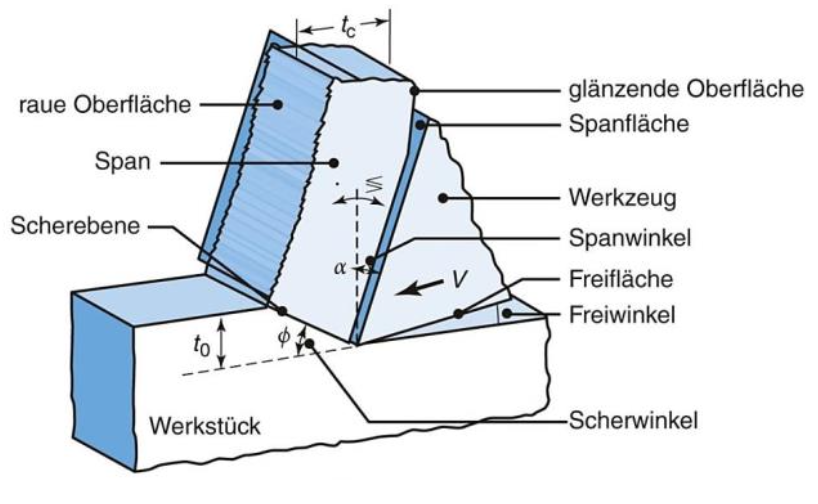
\includegraphics[width=35mm]{src/images/Zerspanvorgang1.png}
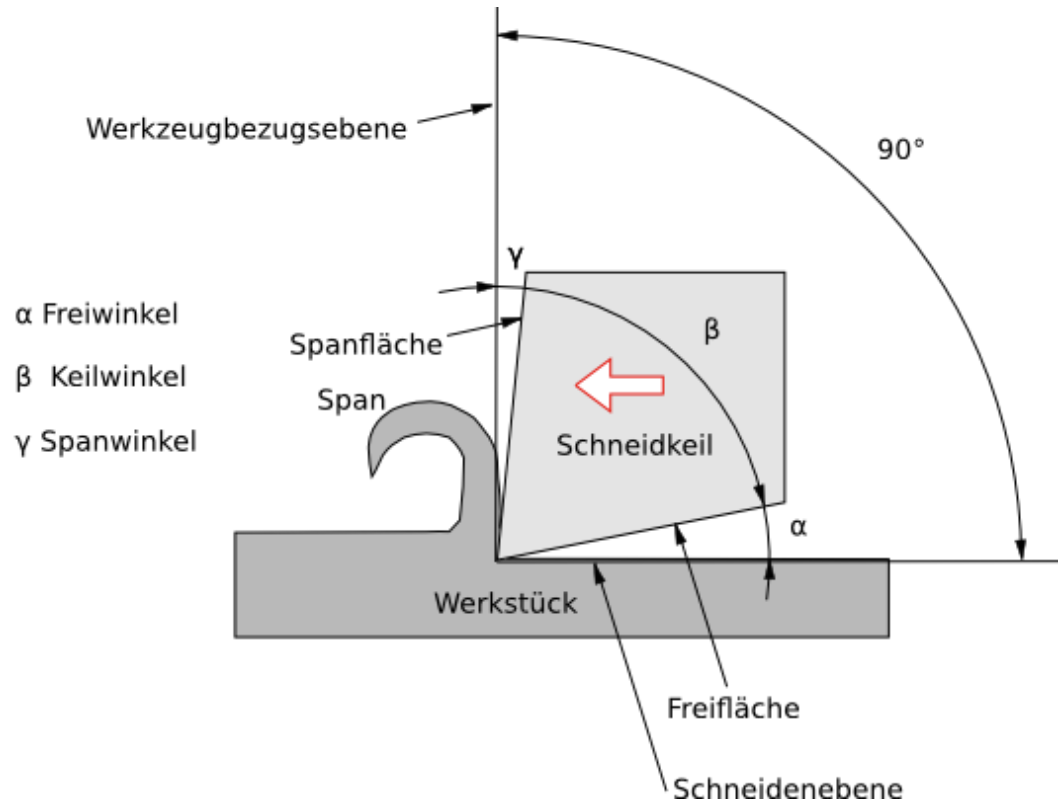
\includegraphics[width= 35mm]{src/images/Zerspanvorgang2.png}\\
\textbf{Verfahren:}\\
Spanen mit geschlossener, meist Kreisförmiger Schnittbewegung 
und beliebiger, quer zur Schnittrichtung liegender Vorschubachse. 
Die Drehachse behält ihre Lage zum Werkstück unabhängig von 
der Vorschubachse bei. \\

\textbf{Kinematische Rauheit, Schnittwinkrl – Drehen:}\\

\begin{minipage}{0.48\linewidth}
    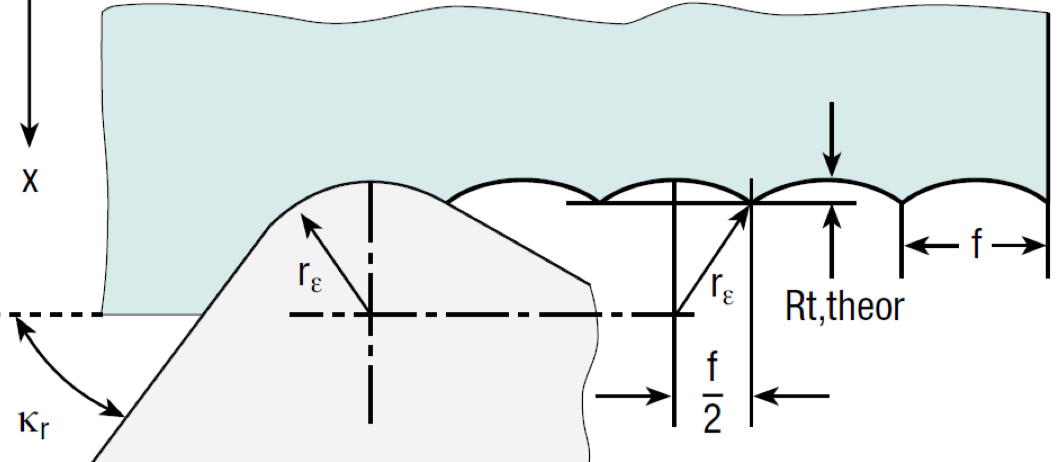
\includegraphics[width=35mm]{src/images/Kinematische Rauheit.jpeg}
    \begin{tiny}
    Theoretische Rauheit:\\ 
    \begin{center}
        \[
            \boxed{        
                R_{t,theor} = \frac{f^2}{8 r_{\varepsilon}}
                }
            \]
    \end{center}
    \end{tiny}
\end{minipage}
\begin{minipage}{0.48\linewidth}
    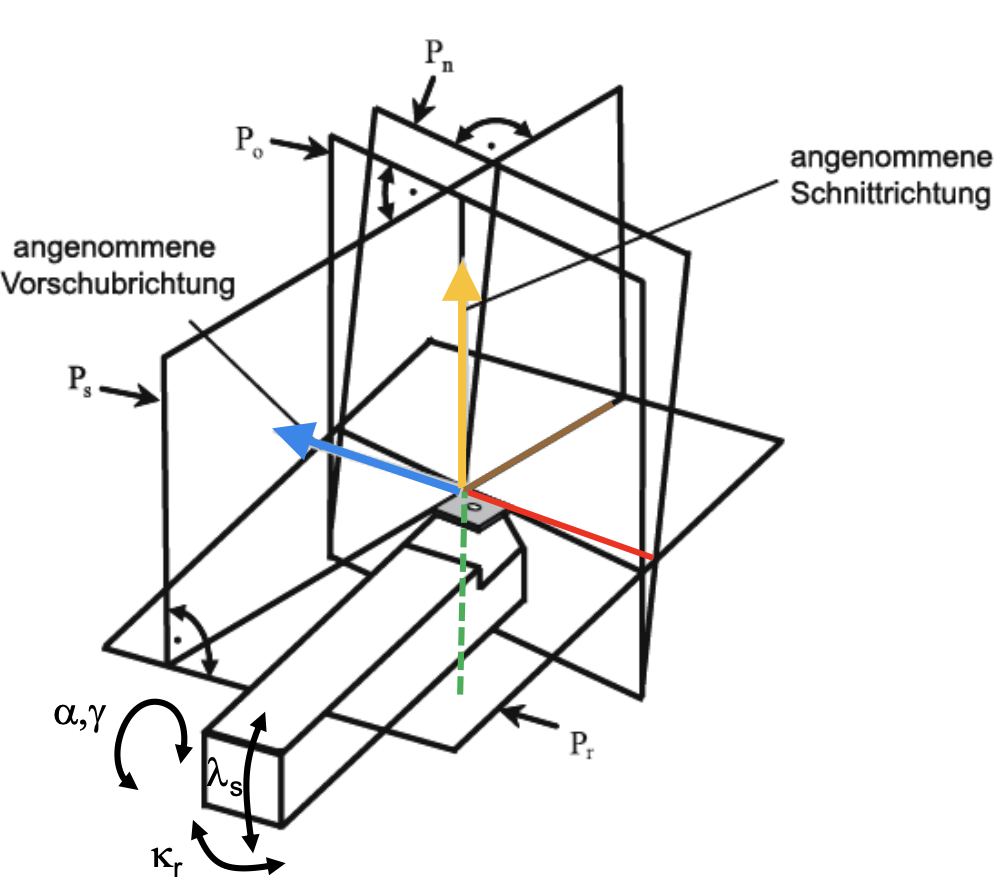
\includegraphics[width=35mm]{src/images/Winkel Drehen.png}\\
\end{minipage}
\\

\textbf{Winkel beim Drehen:}
\begin{itemize}
    \begin{tiny}
        \item Freiwinkel $\alpha$: Winkel zeischen Schneidebene und Freifläche (6°bis 12°)
        \item Keilwinkel $\beta$: Winkel zwischen Span- und Freifläche\\ ($\beta$ = 90 - $\alpha$ - $\gamma$)
        \item Spanwinkel $\gamma$: Winkel zwischen Spanfläche und Werkzeugbezugsebene (-15° bis +25°)
        \item Einstellwinkel $\kappa_r$: Winkel zwischen Hauptschneide und Vorschubrichtung (45° is 110°)
        \item Eckenwinkel $\varepsilon_r$: Winkel zwischen Haupt- und Nebenschneide (35° bis 100°)
        \item Neigungswinkel $\lambda$: Winkel zwischen Hauptschneide und Werkzeugebene (-6° bis +6°)
    \end{tiny}
    \end{itemize}

\textbf{Einfluss des Einstellwinkels:}\\

\begin{minipage}{0.5\linewidth}
    \[
    \boxed{     
        \begin{aligned}
            b &=\frac{a_p}{sin(\kappa_r)}\\
            h &=f\cdot sin(\kappa_r)\\
            A &=a_p\cdot f=b\cdot h
        \end{aligned}
        }
    \]
\end{minipage}
\begin{minipage}{0.5\linewidth}
    \begin{tiny}
    \item $b$: Spanungsbreite
    \item $a_p$: Schnitttiefe
    \item $\kappa_r$: Einstellwinkel
    \item $h$: Spanungsdicke
    \item $f$: Vorschub
    \item $A$: Spanuungsquerschnitt
    \end{tiny}
\end{minipage}\\

\textbf{Ursachen} zur Bildung von \textbf{diskontionuierlichen Spänen:}\\
Spröder Werkstoff, sehr hohe oder niederige Schnitt-\\
geschwindigkeit, grosse Schnitttiefe, geringer Spanwinkel, eiernde (nicht steife) Werkzeugmaschine\\

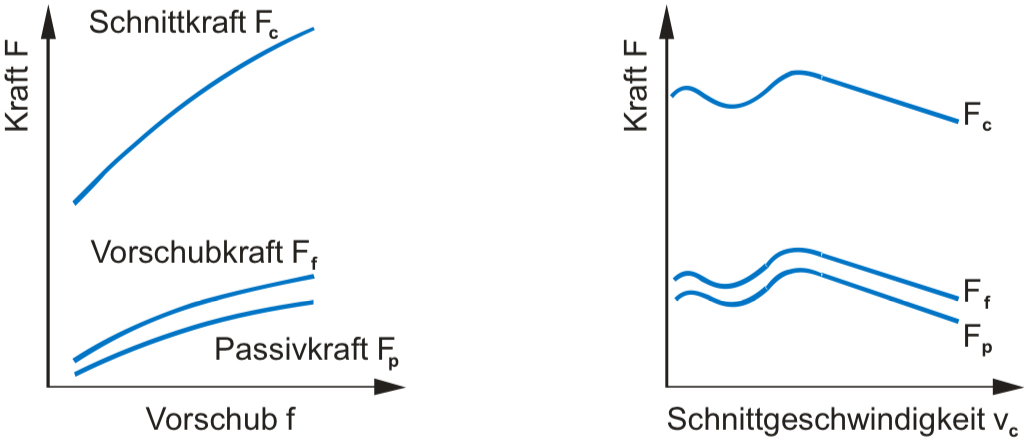
\includegraphics[width=35mm]{src/images/Trennen Diagramme1.jpeg}
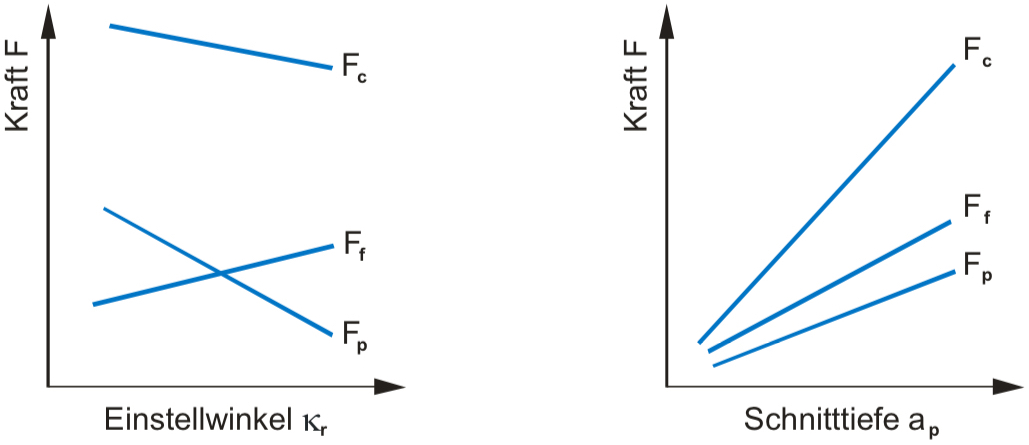
\includegraphics[width=35mm]{src/images/Trennen Diagramme2.jpeg}\\

